\documentclass[12pt,a4paper]{article}
\usepackage{cmap}
\usepackage[slovak]{babel}
\usepackage[utf8]{inputenc}
\usepackage[T1]{fontenc}

\usepackage{amsmath}
\usepackage{amssymb}
\usepackage{lmodern}
\usepackage{indentfirst}
\usepackage{hyperref}
\usepackage{enumitem}
\usepackage{graphicx}
\usepackage{float}
\usepackage{titlesec}

\hypersetup{unicode=true, colorlinks=true, linkcolor=black}

\begin{document}
	
\begin{titlepage}
	\centering
	\vspace{1cm}
	{\scshape\LARGE UnixMotion} \par
	\vspace{1cm}
	{\huge\bfseries Kvantovo-chemické výpočty} \par
	\vspace{2cm}
	{\Large\itshape Jaroslav Ištok \par}
	{\Large\itshape Katarína Fabianová \par}
	{\Large\itshape Dušan Suja \par}
	{\Large\itshape Jerguš Adamec \par}
	\vfill
	\begin{figure}[H]
		\centering
		
\includegraphics[width=0.4\textwidth]{fmfi}
	\end{figure}
	\vspace{2cm}
	{\large FMFI AIN}
\end{titlepage}

\pagebreak

\tableofcontents
\vspace{2cm}
\listoffigures

\pagebreak

\section{Špecifikácia požiadaviek}

\subsection{Úvod}

\subsubsection{Účel}
Špecifikácia obsahuje požiadavky, ktoré bude aplikácia implementovať. Je určená pre každého, kto sa bude podieľať na vývoji. Zadávateľ projektu na základe špecifikácie skontroluje, či výsledná aplikácia bude spĺňať všetky jeho požiadavky. Členovia vývojového tímu ju budú používať pri plánovaní a riadení procesu vývoja. Pomôže im pri ďalšom návrhu aplikácie a neskôr im ju umožní otestovať. Špecifikácia nie je odborným textom, je zrozumiteľná rovnako pre vývojárov aj zadávateľa projektu. Všetky použité odborné termíny sú vysvetlené v sekcii Definície, akronymi a skratky.

\subsubsection{Rozsah projektu}
Projekt sa radí medzi stredne veľké projekty. Jeho vývoj bude prebiehať v časovom horizonte približne pol roka, pričom jeho samotná implementácia bude prebiehať v rozsahu jedného mesiaca. Obsah aplikácie bude pozostávať z častí ako sú crawler, lexer, parser, ORM a jednoduchého, no súčasne intuitívneho grafického užívateľského rozhrania.

\subsubsection{Definície, akronymi a skratky}
\begin{itemize}
	\item Crawler - nástroj, ktorý prelieza adresáre na serveroch a hľadá súbory
	\item Lexer - nástroj, ktorý analyzuje štruktúru súboru (dokumentu)
	\item Parser - nástroj na spracovanie údajov zo súborov
	\item ORM - nástroj na prácu s databázou z programovacieho jazyka
	\item MySQL - relačná (sql) databáza na ukladanie údajov
	\item Apache - webový server, na ktorom bude bežať grafické používateľské rozhranie aplikácie
\end{itemize}

\subsubsection{Odkazy}
\begin{itemize}
	\item Príklad zobrazenia spracovaných dát: \url{http://neon.dpp.fmph.uniba.sk/qch_calcs/index.php}
\end{itemize}

\subsubsection{Prehľad zostávajúcej časti dokumentu}
V nasledujúcich kapitolách nájdete rozširujúce informácie o projekte. Všeobecný popis projektu, perspektívu projektu, podrobný popis funkcionality, účel projektu, charakteristiku cieľových používateľov projektu a ďaľšie.

\subsection{Všeobecný popis}
Aplikácia bude napĺnať databázu zozbieranými údajmi. Bude obsahovať výsledky kvantovo-chemických výpočtov a bude pravidelne aktualizovaná o nové dáta. Aktualizácia dát bude prebiehať automaticky alebo manuálne na vyžiadanie používateľa. Aplikácia bude prístupná len konkrétnym používateľom, ktorí sa budú prihlasovať pomocou prihlasovacieho mena a hesla. Prihlásení používatelia budú môcť vo webovom rozhraní vyhľadávať a filtrovať údaje na základe bázy, metódy merania a ďaľších parametrov. 

\subsubsection{Perspektívny pohľad na projekt}
Projekt bude mať otvorený zdrojový kód. Bude bežať na linuxovom serveri a bude poskytovať webové rozhranie.

\subsubsection{Funkcionalita výslednej aplikácie}
\begin{itemize}
	\item Aplikácia vyhľadá súbory s výsledkami výpočtov z meracích prístrojov, ktoré sú uložené na konkrétnych serveroch. Dáta zo súborov najskôr analyzuje, potom spracuje a uloží ich do databázy.
	\item Aplikácia v pravidelných časových intervaloch, alebo na vyžiadanie používateľa, bude rozširovať databázu o dáta z novopridaných súborov.
	\item Aplikácia poskytne používateľovi jednoduché a intuitívne webové rozhranie, v ktorom bude možné vykonávať požadované operácie nad dátami z databázy, ako je napríklad pokročilé vyhľadávanie na základe rôznych kritérií. Webové rozhranie bude vedieť poskytnúť informácie o určitej molekule, či bola niekedy analyzovaná, akými metódami bola analyzovaná a podobne.
	\item Na prácu s aplikáciou postačí pripojenie na internet a webový prehliadač.
	\item Aplikácia bude chránená heslom a každý používateľ bude mať svoje prihlasovacie údaje, ktoré bude možné zmeniť.
\end{itemize}

\subsubsection{Charakteristika používateľov}
Aplikácia je určená pre chemikov, ktorí pracujú s veľkým množstvom dát z vypočítaných výpočtov a potrebujú v nich mať poriadok. Vzhľadom na povahu aplikácie, nebudú existovať špeciálne používateľské role.

\subsubsection{Všeobecné obmedzenia}
\begin{itemize}
	\item Aplikácia je robená na mieru, takže nemôže si hocikto vytvoriť účet a používať ju.
	\item Na využívanie aplikácie je potrebné mať prístup k internetu a webový prehliadač.
	\item Webové rozhranie zobrazuje len molekuly, ktoré sú uložené v databáze.
	\item Ak je výpočet pre nejakú molekulu neúplný alebo chybný, potom danú molekulu nebude možné zobraziť. Objaví sa iba upozornenie, že dáta z výpočtu nie sú validné.
	\item Ak hľadaná molekula neexistuje v databáze, používateľ má možnosť nahrať súbor s výpočtom pre danú molekulu a v nasledujúcom vyhľadávaní, údaje o molekule budú zobrazené.
\end{itemize}

\subsubsection{Predpoklady a závislosti}
Aplikácia bude bežať na linuxovom serveri. Bude využívať relačnú databázu na ukladanie údajov. Predpokladáme, že nebude mať veľké nároky na procesor a operačnú pamäť. Vzhľadom na povahu dát, ktoré budú v databáze uložené, bude jej veľkosť maximálne niekoľko desiatok megabajtov. Používateľské rozhranie bude bežať na webovom serveri.

\pagebreak

\subsection{Zoznam špecifických požiadaviek na systém}
\begin{enumerate}[label={[\arabic*]}]
	\item {\bf Vyhľadávanie a spracovanie súborov s dátami} 
	\begin{enumerate}
		\item Aplikácie bude vyhľadávať súbory na serveroch ktoré obsahujú výsledky výpočtov z meracích zariadení. vyhľadávať bude na základe prípony v názve súboru. Konkrétne priečinky, ktoré sa budú prehľadávať budú špecifikované v konfiguračnom súbore, ktorý budú editovať používatelia.
		\item Nad zozbieranými súbormi prebehne jednoduchá syntaktická analýza. Tým sa vylúčia súbory, ktoré sú chybné, resp. neobsahujú požadované informácie.
		\item Dáta z validných súborov sa rozparsujú na tokeny, čiže konkrétne údaje, ktoré sa uložia do databázy vo forme tabuliek.
		\item Údaje v databáze budú aktualizované v pravidelných časových intervaloch alebo na vyžiadanie používateľa.
	\end{enumerate}
	\item {\bf Používateľské rozhranie} 
	\begin{enumerate}
		\item Po otvorení stránky sa zobrazí prihlasovacia obrazovka, kde je potrebné zadať prihlasovacie údaje.
		\item V prípade zabudnutia hesla, bude možnosť obnoviť heslo, po zadaní emailu.
		\item Po prihlásení sa zobrazí rozhranie aplikácie, ktoré bude generované dynamicky na základe zvolených kritérii filtrovania údajov, bude obsahovať ovládacie prvky, konkrétne tlačidlo na odhlásenie sa z aplikácie, tlačidlo na aktualizácie údajov v databáze, jednoduchý vyhľadávací box, ktorý bude prehľadávať databázu na základe zvolených kritérii, možnosť editácie konfiguračných súborov a možnosť vykreslenia náhľadu molekuly.
		\item Kritéria, podľa ktorých bude možné vyhľadávať budú napríklad báza, metóda, stechometria (vzorec) molekuly, dátum a ďalšie.
		\item Údaje sa budú zobrazovať v prehľadnej tabuľke.
	\end{enumerate}
\end{enumerate}

\section{Návrh}

\subsection{Diagramy}

\subsubsection{Entitno-relačný diagram}
\begin{figure}[H]
	\centering
	\caption{Entitno-relačný diagram}
	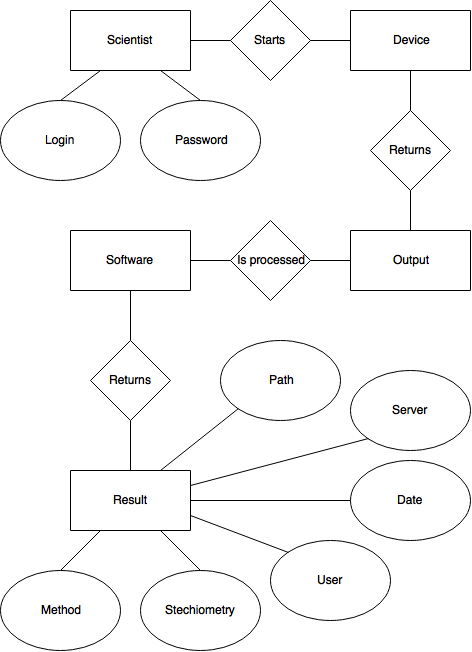
\includegraphics[width=0.65\textwidth]{er_diagram}
	\label{fig:er_diagram}
\end{figure}
\ref{fig:er_diagram}
Entitno-relačný diagram znázorňuje vzťahy (relácie) medzi entitami. Diagram je použitý na modelovanie priestoru domény, pre ktorú sa informačný systém vyvíja (ústav experimentálnej fyziky). Entity sú zakreslené do obdĺžnikov. Vzťahy (relácie) medzi entitami sú v kosoštvorcoch, sú prepojené so všetkými entitami, ktoré do daného vzťahu vstupujú a sú pomenované. Entity majú svoje atribúty, ktoré sú do diagramu zakreslené ako ovály spojené so svojou entitou úsečkou.

\subsubsection{Use-case diagram}
\begin{figure}[H]
	\caption{Use-case diagram}
	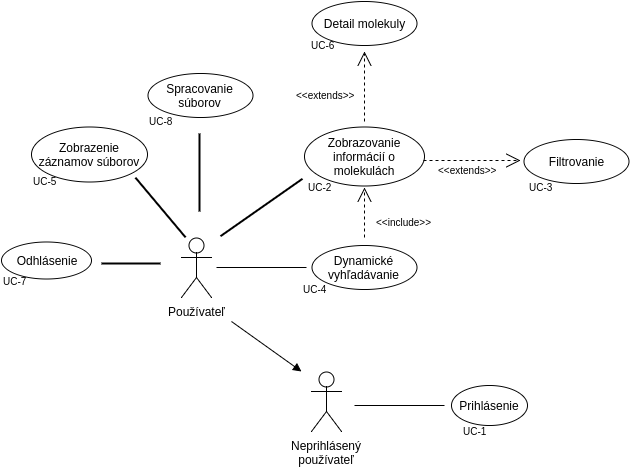
\includegraphics[width=\textwidth]{use-case_diagram}
	\label{fig:use_case}
\end{figure}
\ref{fig:use_case}
Use-case diagram popisuje interakciu používateľov (aktorov) s aplikáciou. Neprihlásený používateľ sa môže prihlásiť. Prihlásený používateľ môže vyhľadávať v databáze výsledkov meraní podľa rôznych kritérií a zobraziť výpis podrobných informácií o danej molekule.

\pagebreak

\begin{enumerate}[label={[UC-\arabic*]}]
	\item {\bf Prihlásenie}
	\begin{itemize}
		\item{\bf Opis: } Po správnom vyplnení údajov doteraz neprihláseného užívateľa prihlási do systému.
		\item{\bf Vstupné podmienky: } Používateľ nie je prihlásený.
		\item{\bf Používatelia: } Používateľmi sú chemici a fyzici.
		\item{\bf Základná postupnosť: }
		\begin{enumerate}[label={\arabic*.}]
			\item Neprihlásený používateľ vyplní meno a heslo.
			\item Neprihlásený používateľ stlačí tlačidlo pre prihlásenie
			\item Systém porovná údaje.
			\item Ak sa údaje zhodujú, systém prihlási používateľa.
		\end{enumerate}
		\item{\bf Alternatívna postupnosť: }
		\begin{enumerate}[label={\arabic*.}]
			\item Neprihlásený používateľ vyplní meno a heslo.
			\item Neprihlásený používateľ stlačí tlačidlo pre prihlásenie
			\item Systém porovná údaje.
			\item Systém používateľa neprihlási do systému.
		\end{enumerate}
	\end{itemize}
	\item {\bf Zobrazovanie informácií o molekulách}
	\begin{itemize}
		\item{\bf Opis: } Zobrazenie základných informácií o molekulách z výpočtov.
		\item{\bf Vstupné podmienky: } Používateľ musí byt prihlásený.
		\item{\bf Používatelia: } Používateľmi sú chemici a fyzici.
		\item{\bf Základná postupnosť: }
		\begin{enumerate}[label={\arabic*.}]
			\item Používateľ sa úspešne prihlási.
		\end{enumerate}
	\end{itemize}
	\item {\bf Filtrovanie}
	\begin{itemize}
		\item{\bf Opis: } Zobrazí len tie molekuly, ktoré vyhovujú podmienkam filtra.
		\item{\bf Vstupné podmienky: } Používateľ musí byť prihlásený.
		\item{\bf Používatelia: } Používateľmi sú chemici a fyzici.
		\item{\bf Základná postupnosť: }
		\begin{enumerate}[label={\arabic*.}]
			\item Používateľ sa úspešne prihlási.
			\item Zadá parametre pre filter.
			\item Zobrazia sa požadované výsledky.
		\end{enumerate}
	\end{itemize}

\pagebreak

	\item {\bf Dynamické vyhľadávanie}
	\begin{itemize}
		\item{\bf Opis: } Pod formulárom sa automaticky zobrazujú tie výsledky, ktoré vyhovujú práve zadávanému reťazcu.
		\item{\bf Vstupné podmienky: } Používateľ musí byť prihlásený.
		\item{\bf Používatelia: } Používateľmi sú chemici a fyzici.
		\item{\bf Základná postupnosť: }
		\begin{enumerate}[label={\arabic*.}]
			\item Používateľ sa úspešne prihlási.
			\item Počas písania do formuláru sa zobrazujú výsledky.
		\end{enumerate}
		\item{\bf Alternatívna postupnosť: }
		\begin{enumerate}[label={\arabic*.}]
			\item Používateľ sa úspešne prihlási.
			\item Počas písania do formuláru nie sú nájdené žiadne výsledky.
		\end{enumerate}
	\end{itemize}
	\item {\bf Zobrazenie záznamov súborov}
	\begin{itemize}
		\item{\bf Opis: } Zobrazí status spracovaných súborov.
		\item{\bf Vstupné podmienky: } Používateľ musí byť prihlásený.
		\item{\bf Používatelia: } Používateľmi sú chemici a fyzici.
		\item{\bf Základná postupnosť: }
		\begin{enumerate}[label={\arabic*.}]
			\item Používateľ sa úspešne prihlási.
			\item Používateľ klikne na tlačítko „Show Report“.
			\item Zobrazia sa požadované výsledky.
		\end{enumerate}
		\item{\bf Alternatívna postupnosť: }
		\begin{enumerate}[label={\arabic*.}]
			\item Používateľ sa úspešne prihlási.
			\item Používateľ klikne na tlačítko „Show Report“.
			\item Nezobrazia sa žiadne záznamy.
		\end{enumerate}
	\end{itemize}
	\item {\bf Detail molekuly}
	\begin{itemize}
		\item{\bf Opis: } Zobrazí detailné informácie o molekule.
		\item{\bf Vstupné podmienky: } Používateľ musí byť prihlásený.
		\item{\bf Používatelia: } Používateľmi sú chemici a fyzici.
		\item{\bf Základná postupnosť: }
		\begin{enumerate}[label={\arabic*.}]
			\item Používateľ sa úspešne prihlási.
			\item Používateľ klikne na tlačidlo „Show details“.
			\item Zobrazí sa nová stránka s detailom molekuly.
		\end{enumerate}
	\end{itemize}
	\item {\bf Odhlásenie}
	\begin{itemize}
		\item{\bf Opis: } Systém používateľa odhlási.
		\item{\bf Vstupné podmienky: } Používateľ musí byť prihlásený.
		\item{\bf Používatelia: } Používateľmi sú chemici a fyzici.
		\item{\bf Základná postupnosť: }
		\begin{enumerate}[label={\arabic*.}]
			\item Používateľ sa úspešne prihlási.
			\item Používateľ klikne na tlačidlo „Odhlásenie“.
			\item Zobrazí sa nová stránka s detailom molekuly.
		\end{enumerate}
	\end{itemize}
	\item {\bf Spracovanie súborov}
	\begin{itemize}
		\item{\bf Opis: } Systém vojde do zadaného priečinka a spracuje v ňom všetky súbory, rozparsuje a uloží ich do databázy.
		\item{\bf Vstupné podmienky: } Používateľ musí byť prihlásený.
		\item{\bf Používatelia: } Používateľmi sú chemici a fyzici.
		\item{\bf Základná postupnosť: }
		\begin{enumerate}[label={\arabic*.}]
			\item Používateľ sa úspešne prihlási.
			\item Používateľ klikne na tlačidlo „Run“.
			\item Zobrazí sa upozornenie, že používateľ spustil akciu.
		\end{enumerate}
	\end{itemize}
\end{enumerate}

\subsubsection{Stavový diagram}
\begin{figure}[H]
	\centering
	\caption{Stavový diagram}
	\includegraphics[width=0.75\textwidth]{state}
	\label{fig:state}
\end{figure}
\ref{fig:state}
Stavový diagram popisuje proces spracovania súboru aplikáciou. Spracovanie sa začína otvorením súboru a jeho následnou prvotnou analýzou (validáciou). V prípade, že súbor nie je validný, tak sa nepokračuje ďalej v jeho spracovaní. V prípade, že súbor je validný sa zistí, či má súbor windowsový alebo linuxový formát. Tieto dva formáty sa líšia vnútornou štruktúrou a teda aj spôsobom spracovania. Zo súboru sa následne vyparsujú potrebné dáta a spracovanie súboru skončí jeho zatvorením. 

\subsubsection{Sekvenčný diagram - spracovanie súboru}
\begin{figure}[H]
	\caption{Sekvenčný diagram - spracovanie súboru}
	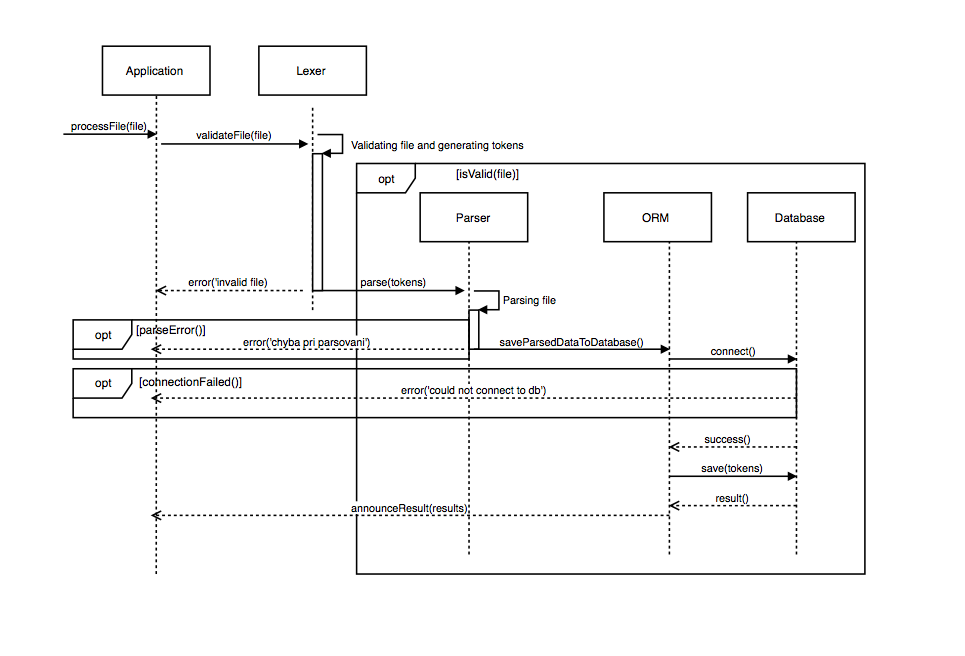
\includegraphics[width=\textwidth]{sequence_file}
	\label{fig:seq}
\end{figure}
\ref{fig:seq}
Diagram popisuje komunikáciu komponentov našej aplikácie počas spracovania súboru. Na začiatku aplikácia pošle lexeru požiadavku na validáciu súboru. Lexer súbor zvaliduje a rozparsuje na tokeny, v prípade chyby, pošle hlavnému programu správu s chybou. Tokeny pošle parseru, ktorý ich rozparsuje. Dáta z parseru sa pošlú ORM-ku, ktoré sa pripojí k databáze a uloží do nej naparsované dáta. Na konci pošle správu o úspechu, resp. neúspechu celej operácie do hlavného programu, ktorý ju spracuje.

\subsubsection{Sekvenčný diagram -  pripojenie k databáze}
\begin{figure}[H]
	\caption{Sekvenčný diagram - pripojenie k databáze}
	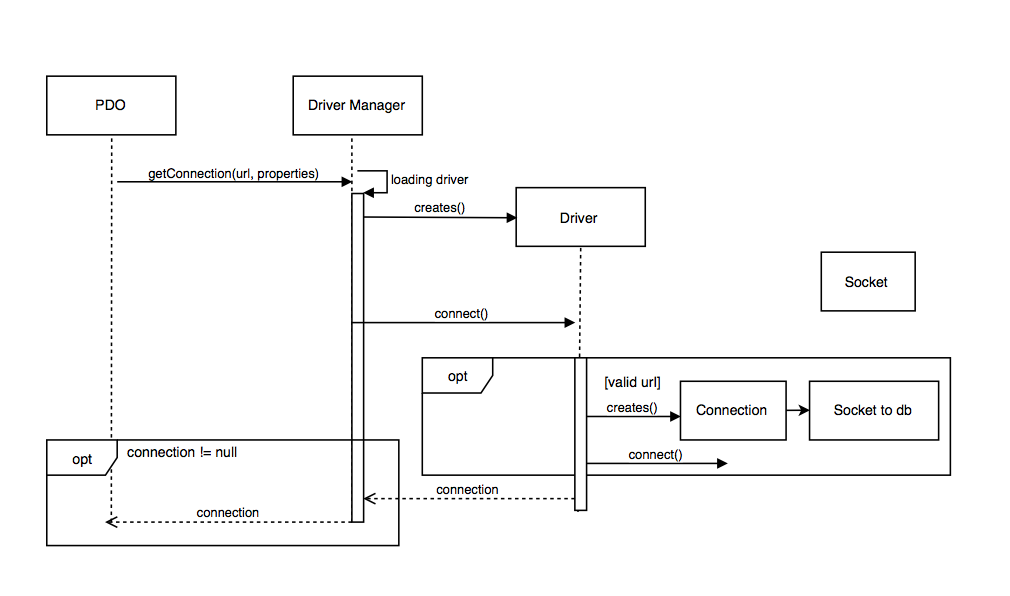
\includegraphics[width=\textwidth]{db}
	\label{fig:db}
\end{figure}
\ref{fig:db}
Diagram popisuje proces pripojenia k databáze. Knižnica PDO pošle požiadavku na získanie spojenia k databáze driver manageru. Ten načíta driver, vyberie správny a vytvorí jeho inštanciu. Driver sa následne pokúsi vytvoriť spojenie k databáze tým, že sa pokúsi pripojiť na socket. V prípade neúspechu sa o ňom pošle správa do PDO. V prípade úspešného pripojenia na socket sa vráti spojenie k databáze do PDO.

\subsubsection{Dátový model}
\begin{figure}[H]
	\caption{Dátový model}
	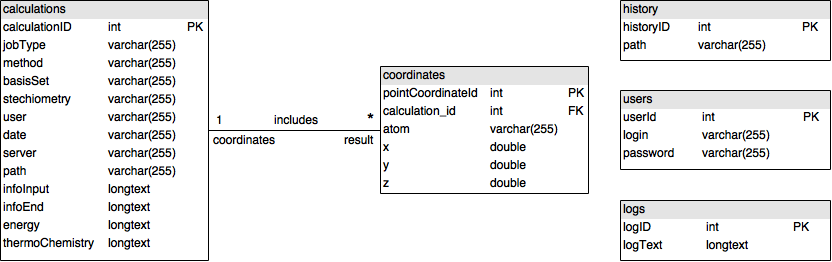
\includegraphics[width=\textwidth]{datovy_model}
	\label{fig:datovy_model}
\end{figure}
\ref{fig:datovy_model}
Dátový model popisuje štruktúru databázy.
\begin{itemize}
	\item{\bf Calculations} \par
	Tabuľka calculations obsahuje zoznam výsledkov výpočtov. Výsledky výpočtov majú priradené id, plniace funkciu primárneho kľúča (calculationID), spôsob testovania vzorky (jobType), metódu testovania vzorky (method), iniciálnu konfiguráciu (basisSet), zjednodušený chemický vzorec testovanej vzorky (stechiometry), používateľa, spúšťajúceho testovanie vzorky (user), dátum testovania vzorky (date), meno servera, ukladajúceho daný výsledok výpočtu (server), cestu k súboru daného výsledku výpočtu (path), bližšie nešpecifikované, zadávateľom požadované údaje (infoInput), (infoEnd), energiu (energy) a termochémiu (thermoChemistry).
	\item{\bf Coordinates} \par
	Tabuľka coordinates obsahuje zoznam súradníc jednotlivých atómov. Súradnice atómov majú priradené id, plniace funkciu primárneho kľúča (pointCoordinateId), atóm, ktorému prislúchajú (atom), súradnicu x (x), súradnicu y (y) a súradnicu z (z).
	\item{\bf Users} \par
	Tabuľka users obsahuje zoznam používateľov. Používatelia majú priradené id, plniace funkciu primárneho kľúča (userId), meno, pod ktorým sa prihlasujú (login) a heslo, s ktorým sa prihlasujú (password).
	
\pagebreak
	
	\item{\bf History} \par
	Tabuľka history obsahuje zoznam spracovaných súborov. Spracované súbory majú priradené id, plniace funkciu primárneho kľúča (historyID) a cestu, ktorá popisuje ich umiestnenie (path).
	\item{\bf Logs} \par
	Tabuľka logs obsahuje zoznam chybových správ. Chybové správy majú priradené id, plniace funkciu primárneho kľúča (logID) a text, ktorý je ich obsahom (logText).
	\item{\bf Popis vzťahov medzi entitami} \par
	Tabuľky users, history a logs sa neviažu na žiadnu tabuľku. Tabuľka coordinates sa viaže na tabuľku calculations tak, že jedna súradnica atómu je obsiahnutá v práve jednom výsledku výpočtu, pričom jeden výsledok výpočtu môže obsahovať niekoľko súradníc atómov.
\end{itemize}

\pagebreak

\subsubsection{Komponentný diagram}
\begin{figure}[H]
	\centering
	\caption{Komponentný diagram}
	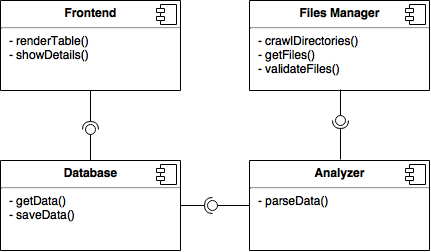
\includegraphics[width=0.7\textwidth]{komponentny_diagram}
	\label{fig:komponentny_diagram}
\end{figure}
\ref{fig:komponentny_diagram}
Komponentný diagram popisuje dekompozíciu projektu na moduly.
\begin{itemize}
	\item{\bf Frontend} \par
	Komponent frontend má na starosti sprístupnenie viditeľného obsahu aplikácie (napr. rozloženie stránky, užívateľské rozhranie, grafika, text) používateľovi.
	\item{\bf Database} \par
	Komponent database má na starosti pripojenie k databáze a prácu s ňou. Získava a ukladá údaje.
	\item{\bf Analyzer} \par
	Komponent analyzer má na starosti rozparsovanie súboru s výsledkami výpočtov z meracích prístrojov. Dostane súbor a povyberá z neho potrebné údaje.
	\item{\bf Files Manager} \par
	Komponent files manager má na starosti vyhľadávanie a kontrolovanie valídnosti súborov uložených na konkrétnych serveroch. Dostane cesty k priečinkom, v ktorých nájde súbory so zadanými koncovkami. Následne zistí či nájdené súbory majú validnú štruktúru.
	\item{\bf Popis toku údajov medzi komponentami} \par
	Tok údajov medzi komponentami je znázornený úsečkami so zodpovedajúcimi symbolmi. Kalichom na strane prijímateľa a guličkou na strane poskytovateľa.
\end{itemize}

\subsubsection{Triedny diagram}
\begin{figure}[H]
	\caption{Triedny diagram}
	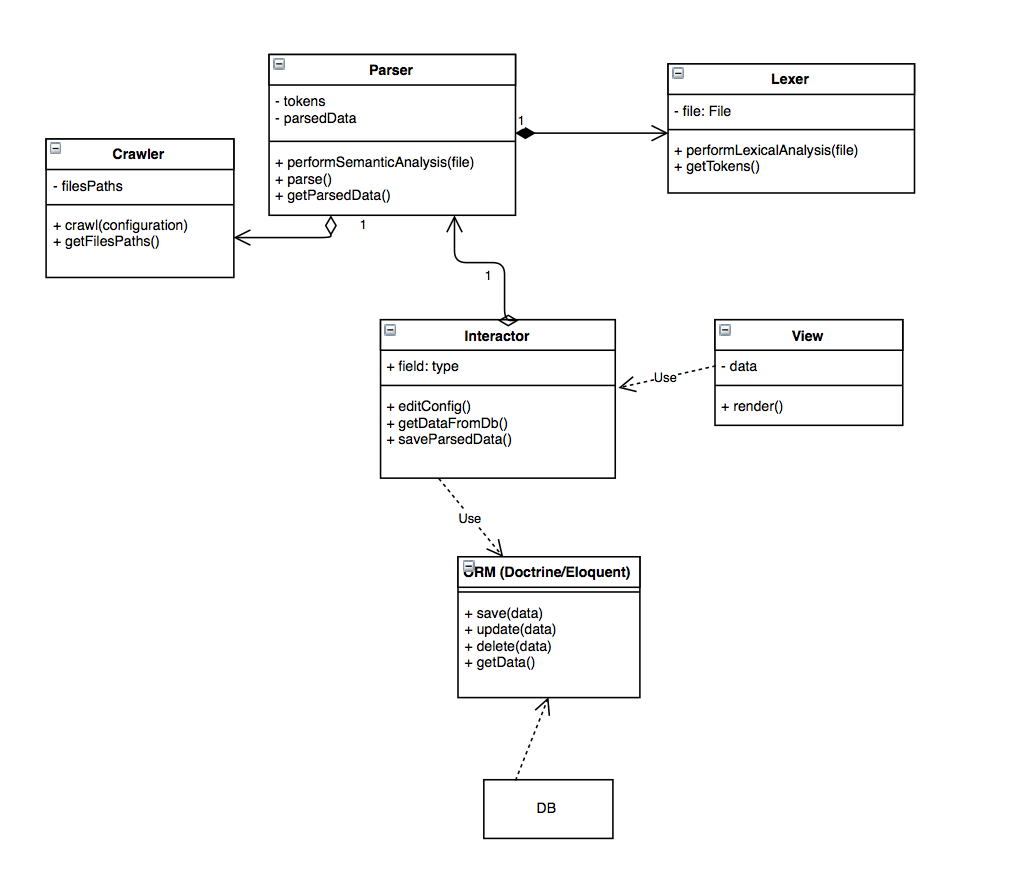
\includegraphics[width=\textwidth]{class_diagram}
	\label{fig:class_diagram}
\end{figure}
\ref{fig:class_diagram}
Triedny diagram modeluje jednotlivé triedy a vzťahy medzi nimi. Každá entita triedneho diagramu popisuje triedu, jej základné atribúty a metódy. Medzi triedami sú šípky, ktoré reprezenutujú jednotlivé vzťahy. Parser bude používať Crawler na vyhľadanie súborov a rovnako bude používať aj Lexer, pomocou, ktorého spraví lexikálnu analýzu súboru. Interactor bude akési spojítko jednotlivých hlavných častí aplikácie. View-u bude poskytovať dáta na zobrazenie a Parseru poskytne prístup k databáze.

\subsection{Používateľské rozhranie}
Používateľké rozhranie aplikácie je navrhnuté jednoducho podľa požiadaviek zadávateľa projektu.
\begin{figure}[H]
	\caption{Obrazovka s prihlásením}
	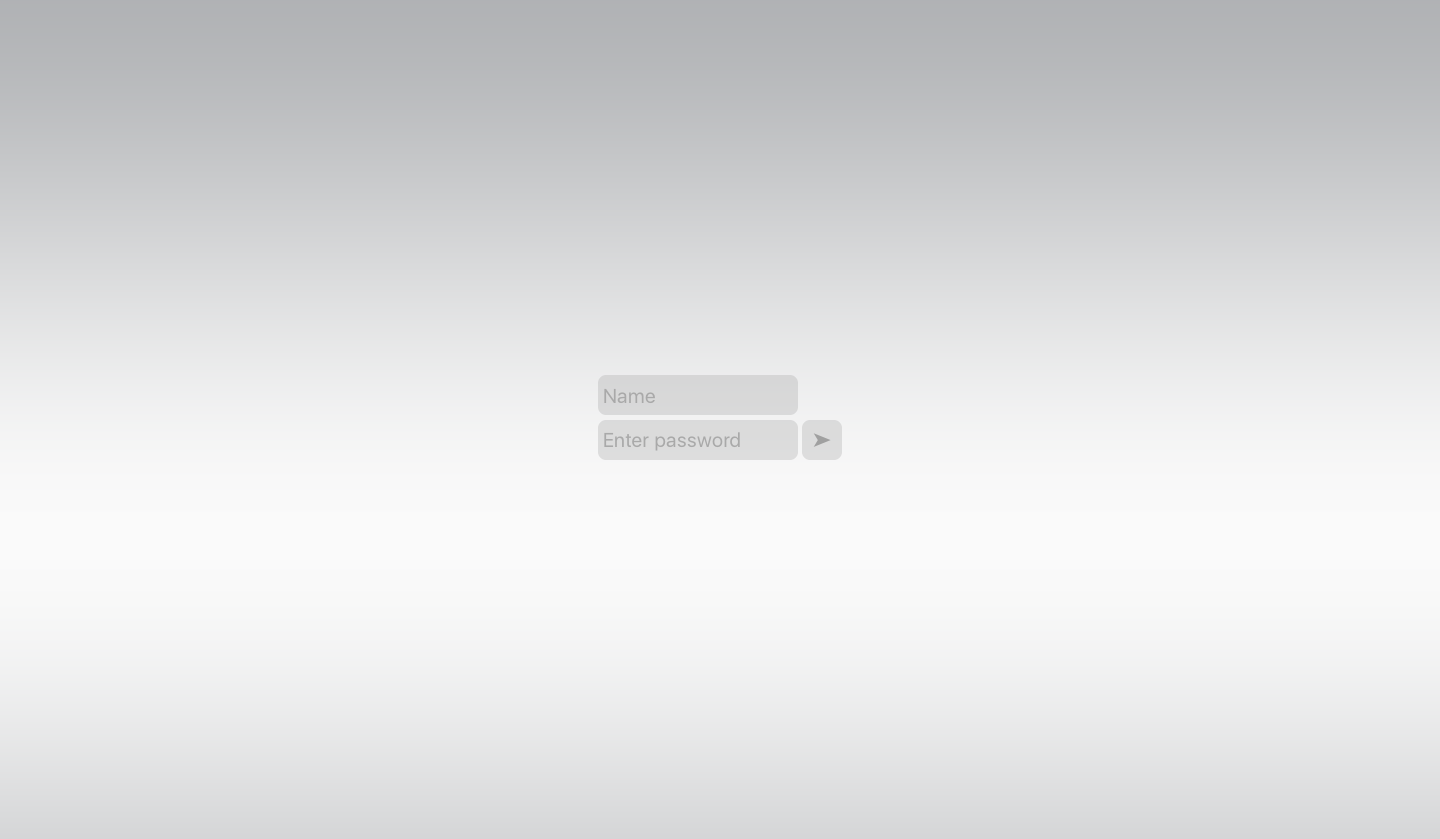
\includegraphics[width=\textwidth]{login}
	\label{fig:ui1}
\end{figure}
\ref{fig:ui1}
Úvodná obrazovka s prihlásením pozostáva z prihlasovacieho formuláru tvoreného textovými poľami, určenými pre zadanie používateľského mena a používateľského hesla, slúžiacimi na identifikáciu jednotlivých vybraných používateľov.
\begin{figure}[H]
	\caption{Obrazovka s tabuľkou výpočtov}
	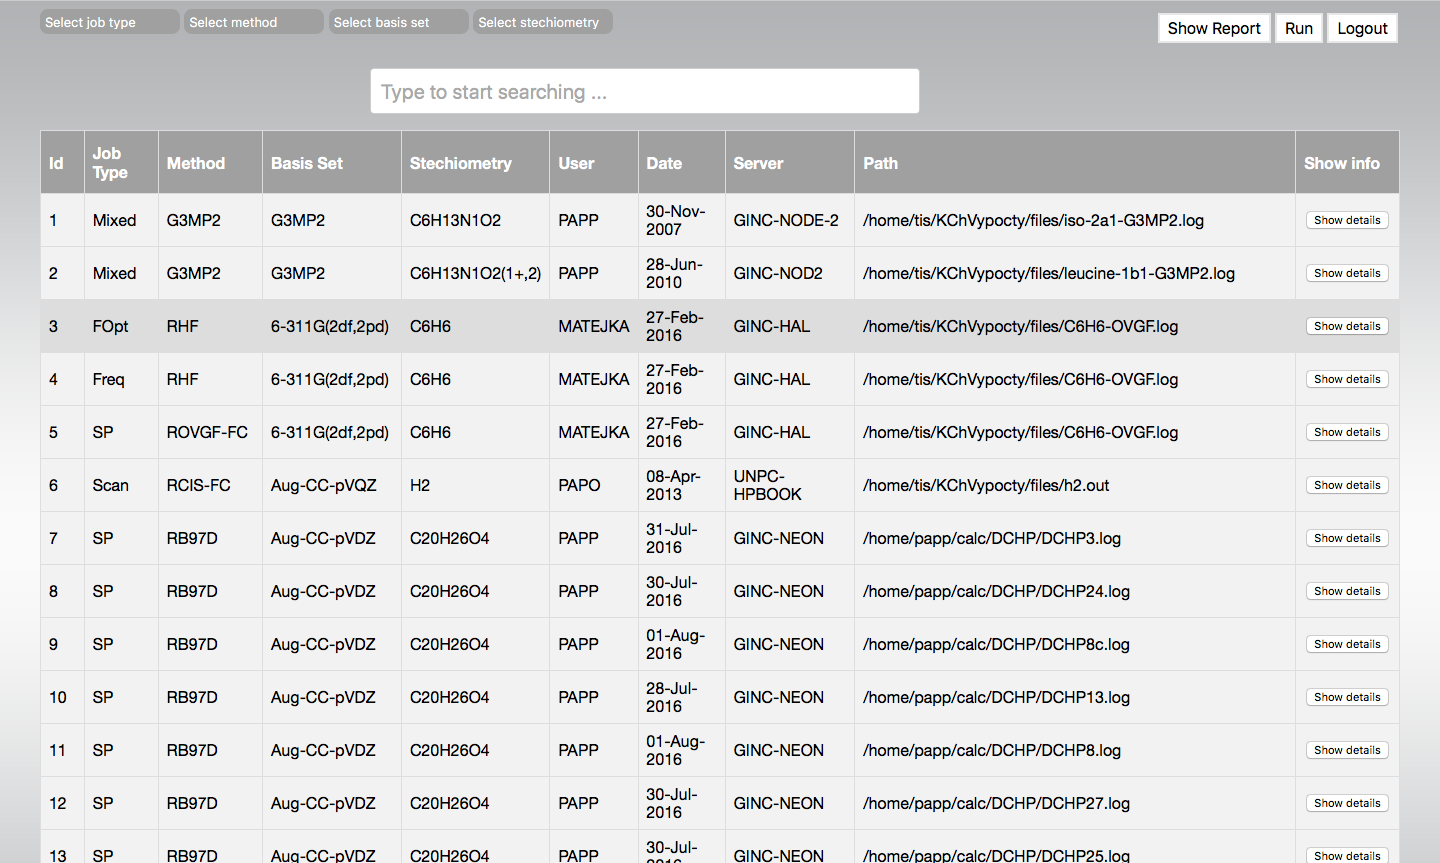
\includegraphics[width=\textwidth]{table}
	\label{fig:ui2}
\end{figure}
\ref{fig:ui2}
Po prihlásení sa zobrazí hlavná stránka. Nachádza sa na nej tabuľka všetkých údajov, ktoré sú uložené v databáze. Medzi údajmi je možné vyhľadávať pomocou interaktívneho vyhľadávacieho pola alebo ich filtrovať pomocou filtrov. Nachádza sa tam aj tlačidlo na zobrazenie logu, spustenie novej analýzy súborov a odhlásenie používateľa.
\begin{figure}[H]
	\caption{Obrazovka s výpočtom}
	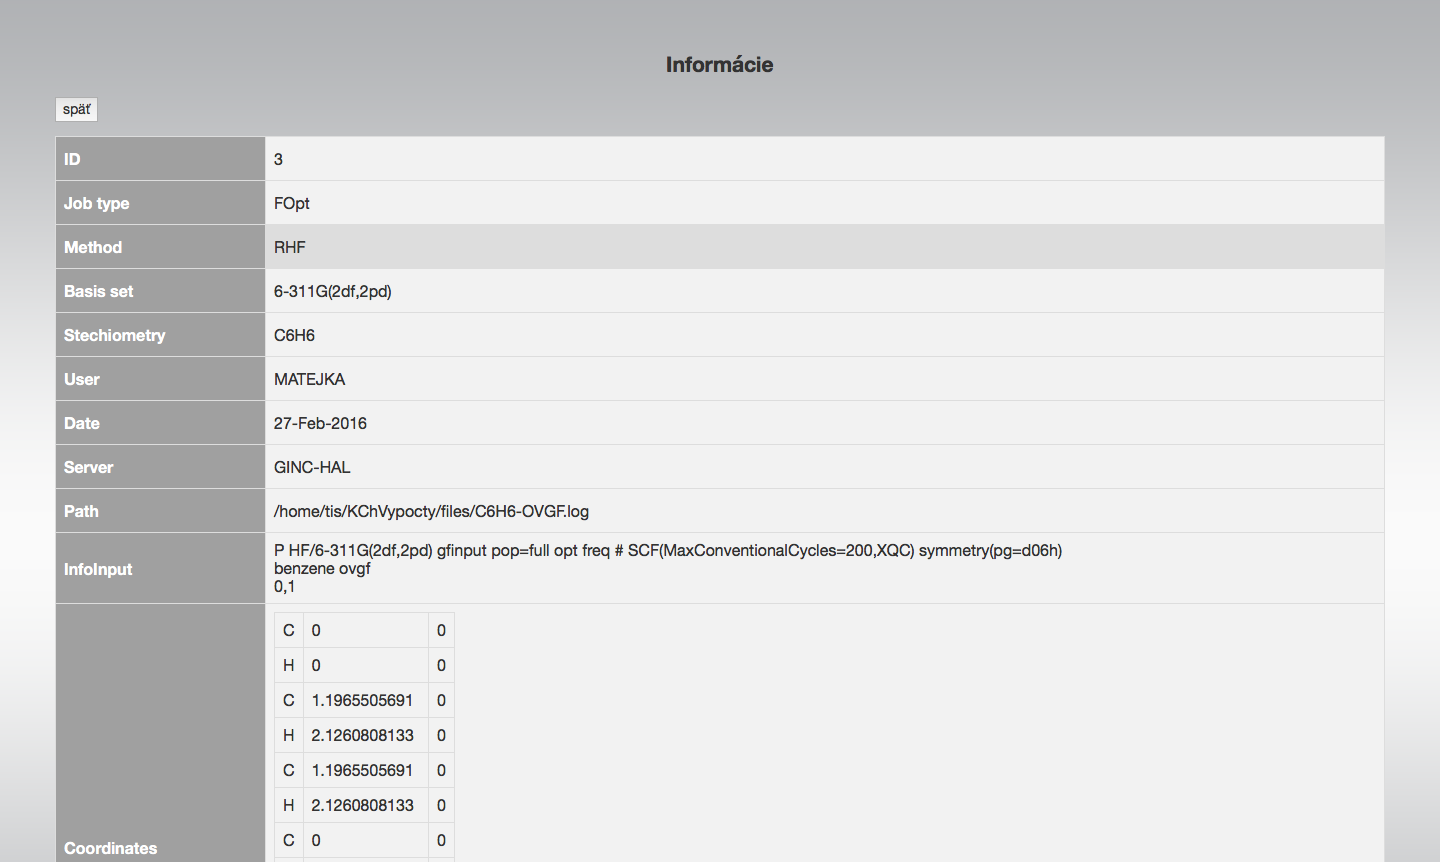
\includegraphics[width=\textwidth]{item}
	\label{fig:ui3}
\end{figure}
\ref{fig:ui3}
Pri každom výpočte zobrazenom v tabuľke sa nachádza tlačidlo “Show details”. Kliknutím na toto tlačidlo sa zobrazí detailný výpis všetkých informácií o výpočte v prehľadnej tabuľke.

\pagebreak

\subsection{Analýza technológií}

\subsubsection{Výber programovacieho jazyka}
Pri výbere programovacieho jazyka sme sa rozhodovali medzi Python-om a PHP. Vybrali sme si PHP, pretože je pre tento projekt najvhodnejší. Medzi výhody, ktoré nám ponúka pri vývoji patria napríklad:
\begin{itemize}
	\item Patrí medzi najpoužívanejšie jazyky vo webových aplikáciach.
	\item Je predinštalovaný na serveri, na ktorom bude bežať aj naša aplikácia.
	\item Plne podporuje objektovo orientované programovanie.
	\item V PHP je na výber veľa kvalitných frameworkov na prácu s databázou.
	\item Vieme s ním efektívne pracovať.
\end{itemize}
Python je náročnejšie nakonfigurovať na webovom serveri, kde pravdepodobne nebudeme mať možnosť inštalácie nového softwéru a oproti PHP ponúka len málo výhod pre náš projekt. Žiadnu podstatnú výhodu nám Python neponúka.

\subsubsection{Výber databázového systému}
Pri výbere databázového systému sme sa rozhodovali medzi Mysql a PostgreSql. PostgreSql ponúka veľa pokročilých funkcií, ako napríklad rekurzívne dopyty, pohľady. Naša aplikácia bude obsahovať jednoduchú databázu s malým počtom tabuliek a tieto pokročilé funkcie nevyužijeme. Preto sme si vybrali mysql databázu, ktorá je predinštalovaná na serveri a jej databázové enginy sú optimalizované pre webové aplikcie.

\subsubsection{Výber ostatných technológií}
\begin{itemize}
	\item{\bf HTML} \par
	Hypertextový značkový jazyk (HyperText Markup Language; HTML) je značkový jazyk určený na vytváranie webových stránok a iných informácií zobraziteľných vo webovom prehliadači. HTML kladie dôraz skôr na prezentáciu informácií (odseky, fonty, váha písma, tabuľky atď.) ako na sémantiku (význam slov) a umožňuje vytvárať dokumenty obsahujúce text, hypertextové odkazy, multimediálny a iný obsah, formuláre, skripty a metainformácie prehliadateľné v tzv. webovom prehliadači. Jazyk HTML je textový, teda umožňuje čítanie a upravovanie priamo v textovom editore. V projekte bude použitý pri tvorbe webových dokumentov z hľadiska ich obsahu, štruktúry.
	\item{\bf CSS} \par
	Kaskádové štýly (Cascading Style Sheets; CSS) je všeobecné rozšírenie HTML. CSS je jednoduchý mechanizmus na vizuálne formátovanie internetových dokumentov. Pomocou kaskádových štýlov sa vytvárajú štruktúrované dokumenty, teda oddeľuje sa obsah dokumentu (HTML) od jeho vzhľadu (CSS). Získa sa tým prehľadný a jednoduchý kód. CSS je možné presunúť do externých súborov, zmenší sa tým dátová veľkosť a dá sa jedným súborom zmeniť celý štýl stránky, pričom sa nezaručuje rovnaké vykresľovanie vo všetkých prehliadačoch, vzhľadom k rôznym interpretáciam CSS rôznymi prehliadačmi. V projekte budú použité pri tvorbe webových dokumentov z hľadiska ich výzoru.
	\item{\bf JavaScript} \par
	JavaScript je skriptovací programovací jazyk využívaný najmä na vytváranie dynamického obsahu webových stránok. V projekte bude použitý pri tvorbe webových dokumentov z hľadiska ich dynamického obsahu a reagovania na vstup používateľa.
	\item{\bf AJAX} \par
	AJAX (Asynchronous JavaScript + XML) je súhrnné označenie pre technológie vývoja interaktívnych webových aplikácií, ktoré umožňujú meniť obsah stránok bez potreby ich kompletného znovunačítania zo servera. V porovnaní s klasickými webovými aplikáciami môžu AJAX-ové aplikácie pri vhodnom návrhu poskytovať používateľsky komfortnejšie prostredie, vyžadujú však použitie moderných webových prehliadačov. AJAX nie je samostatný programovací jazyk ani technológia sama o sebe. Je to kombinácia HTML a CSS pre značkovanie a štýlovanie informácií pri zobrazení, DOM spojeného s JavaScriptom pre dynamické zobrazenie a interakciu s prezentovanou informáciou, metódy pre výmenu dát medzi prehliadačom a serverom, bez nutnosti obnovovať zobrazovanú stránku a formátu pre dáta poslané prehliadaču, ktoré môžu byť dynamicky vytvorené skriptom na strane serveru (bežné formáty zahŕňajú XML, predformátované HTML, plain text a JavaScript Object Notation, JSON). V projekte budú použité pri zmene obsahu webových dokumentov bez potreby ich kompletného znovunačítania zo servera.
\end{itemize}

\subsection{Testovacie scenáre}

\subsubsection{Existencia súboru}
Otestovať existenciu súboru a jeho korektné otvorenie. Ak funkcia dostane cestu korektného súboru, so súborom sa dá ďalej pokračovať. V opačnom prípade funkcia súbor zahodí a nepokračuje sa v ďalšom spracovávaní.

\subsubsection{Crawler}
Otestovať funkcionalitu Crawlera. Používateľ pridá nové súbory v používateľskom rozhraní. Crawler má nájsť novopridané súbory a aktualizovať databázu. 

\subsubsection{Validnosť súboru}
Otestovať validnosť súboru. Ak funkcia dostane validný súbor (je v požadovanom formáte), pokračuje sa ďalej v procese. V opačnom prípade, ak funkcia dostane nevalidný vstup (súbor je v zlom formáte), ďalej sa nepokračuje a funkcia súbor zahodí.

\subsubsection{Rozlišovanie linuxových a windowsových súborov}
Otestovať rozlišovanie medzi linuxovým a windowsovým súborom (rozdiel je v type súboru a v pár znakoch). Funkcia rozlíši, či dostala na vstup linuxový alebo windowsový súbor a následne sa súbor parsuje podľa linuxového alebo windowsového formátu.  

\subsubsection{Databáza}
Otestovať pridávanie nových prvkov do databázy. Pridá sa nový korektný súbor a následne treba zistiť, či sa pridal aj do databázy. Pridá sa nový nekorektný súbor a následne treba skontrolovať, či sa údaje zo súboru nepridali do databázy.

\subsubsection{Prihlásenie}
Otestovať správne prihlásenie používateľa. V používateľskom rozhraní sa zadajú správne prihlasovacie údaje (meno a heslo), očakávaným výsledkom je úspešné prihlásenie sa na stránku. Zadajú sa nesprávne prihlasovacie údaje (nesprávne meno alebo nesprávne heslo alebo oboje), aplikácia zobrazí chybovú hlášku zlého prihlásenia a stránka nie je dostupná.

\subsubsection{Vyhľadávanie v databáze}
Otestovať správnosť vyhľadávania v databáze. Zadajú sa parametre, podľa ktorých sa v databáze nachádzajú nejaké molekuly, aplikácia zobrazí všetky molekuly korektne.

\subsubsection{Pridávanie nových súborov}
Otestovať aktualizovanie databázy. Po pridaní nového súboru cez používateľské rozhranie, sa automaticky aktualizuje databáza a pri vyhľadávaní molekúl sa zobrazia aj najnovšie pridané údaje.

\end{document}